\documentclass[a4paper,10.0pt,twoside]{npr}

\usepackage{multicol,graphicx,lastpage,footmisc,fancyhdr,paralist,
tabularx,array,booktabs,caption,multirow,upgreek,mathrsfs,gensymb,color}
\usepackage[fancyhdr,space,fntef,fontset=ubuntu]{ctex}
\usepackage{amssymb,bm,mathrsfs,bbm,amscd}
\usepackage{flushend,cuted}
\usepackage{refcount}
\usepackage{savesym}
\usepackage{textcomp}
\usepackage[tbtags]{amsmath}  %
\savesymbol{iint}
\usepackage{amstext} %数学宏包文本命令
\usepackage{balance} %版心底部对齐

\flushbottom      %版心底部对齐
\setcounter{section}{0}
\begin{document}
%\begin{CJK*}{GBK}{\song}{\wuhao}{\rm}

%___________________________________________________________________________________
\def\rd{{\rm d}}

\newcommand{\RM}{\ensuremath{\mathrm}}   %正体 既可用于文本模式也可用于数学模式
\newcommand{\dif}{\mathrm{d}}  %直立体d
\newcommand{\me}{\mathrm{e}}  %直立体e
\newcommand{\mi}{\mathrm{i}}  %直立体i
\newcommand{\mj}{\mathrm{j}}  %直立体j
\newcommand{\afrac}[2]{\dfrac{\,#1\,}{\,#2\,}}  %略长分数线
\newcommand{\nn}{\nonumber}  %公式无编号
\newcommand{\nt}{\noindent}
\newcommand{\OO}{~\text{。}}
\newcommand{\PP}{~\text{,}}
\newcommand{\OP}{~\text{;}}
\newcommand{\LT}{\left}
\newcommand{\RT}{\right}

%___________________________________________________________________________________

\balance
\fancypagestyle{myfoot}
{%
\fancyhf{}
\fancyhead[c]{\wuhao\song 高~等~核~物~理~实~验}
\renewcommand{\headrule}{\vskip 2pt
\hrule height0.4pt width\headwidth \vskip1pt
\hrule height0.4pt width\headwidth \vskip-1.8pt}
}%
\thispagestyle{myfoot}

%%%%%%%%%%%%%%%%%%%%%%%%%%%%%%%%%%%%%%%%%%%%%%%%%%%%%
%    奇偶页眉
%%%%%%%%%%%%%%%%%%%%%%%%%%%%%%%%%%%%%%%%%%%%%%%%%%%%%
\pagestyle{fancy}
\fancyhead{}
\fancyhead[ce]{\xiaowu\song \hspace{0.5em}高~等~核~物~理~实~验}
%\fancyhead[ro,le]{\xiaowuhao \hspace{0.5em}\textbf{\textperiodcentered}\;\thepage\;\textbf{\textperiodcentered}\hspace{0.5em}}
%\fancyhead[ce]{\xiaowu\song 粒~子~物~理~与~原~子~核~物~理~专~题~实~验}
%\fancyhead[re]{\xiaowu\song \hspace{0.5em}第\;31\;卷\hspace{0.5em}}
\fancyfoot[ce,co]{}
\renewcommand{\headrule}{\vskip 2pt
\hrule height0.4pt width\headwidth}


\setcounter{page}{001}%
\fancyhead[co]{\xiaowuhao\song  乔颢:NaI(Tl)闪烁谱仪测定$\gamma$射线的能量}    %奇页页眉
\begin{center}
\title{%
\xiaoerhao \bf  %章标题为两行时改为 \exiaoer
NaI(Tl)闪烁谱仪测定$\gamma$射线的能量\\[-5mm]}
\maketitle
\large \fs
乔颢$^{^1}$\\[2mm]

\xiaowu \song
1. 北京大学物理学院,海淀区 北京 100871;\\[4mm]

 
\footnotetext[0]{{\bf 作者简介:}~~\begin{minipage}[t][4.2mm]{149mm}\song
乔颢,E-mail: i@catofes.com
\end{minipage} }
%\footnotetext[0]{{\bf 通信作者:}\song ~~E-mail: xxx@xxx.xxx }%通信作者为第一作者时不要此项

\parbox{158mm} {
\zywu{\bf 摘要:}~~\fs
该实验通过NaI(Tl)闪烁体谱仪测量得到了$^{137}$Cs的全能谱,并通过其全能峰,反散射峰以及$^{60}$Co的两个光电峰对闪烁谱仪进行了标定。得到的标定曲线为$  E(MeV) = 0.206 U(V) - 0.047 $。同时利用多道再次测量并验证了Cs的能谱图以及Cs和Co的混合能谱图。\\

{\bf 关键词:}~~\fs NaI(Tl)闪烁谱仪, $\gamma$射线, $\gamma$能谱 , 能量刻度}\\
\end{center}
%%%%6.正文
\vspace{5mm}
%%%%6.正文
\setcounter{section}{0}
\begin{multicols}{2}
%----------------
%____________________________________________________________________________
%%%%以上请不要改动%%%%%%%%%%%%%%%%%%%%%%%%%%%%%%%%%%%%%%%%%%%%

\section{引言}    %1
\vspace*{-1mm}
\song\wuhao
闪烁体探测器是一种测量辐射粒子能量的主要方法,它利用某些物质在射线的作用下会发光的特性来探测射线。大部分闪烁体探测器属于信号探测器,在核物理实验中主要用来测量粒子的辐射强度以及能谱。本实验中采用的NaI探测器是无机发光体探测器,对$\gamma$射线就有较高的探测效率。

NaI闪烁谱仪就是使用含(Tl)的NaI晶体作为闪烁体的探测器,配合后续电子学器件例如放大器的多道等,所组成的谱仪。它探测效率较高,发光衰减时间较短,具有较好的时间分辨和能量分辨。通过NaI闪烁体频谱仪,我们得以细致的研究物质的$\gamma$衰变,能够对对$\gamma$能谱进行定量测量从而更好地理解$\gamma$射线与物质作用的机理。
\section{实验}
\subsection{实验介绍及原理}
$\gamma$粒子与物质发生的相互作用主要是光电效应,康普顿散射以及正负电子对这三种相互作用。

光电效应中入射的$\gamma$粒子将所有能量交给原子中的束缚电子,将束缚电子打出形成光电子。光电子的能量满足
\begin{equation}
   E_{e}= E_\gamma - E_i \approx E_\gamma
\end{equation}
式子中$E_{e}$是出射电子能量,因为电离能$E_i$很小,所以出射电子能量接近于入射的$\gamma$能量$E_\gamma$。当吸收体中发生光电效应时,$\gamma$所有的能量都交予光电子,在然后被闪烁材料吸收发出光。这在能谱上对应的就是全能峰。

当$\gamma$射线与核外自由电子进行碰撞时会发生康普顿散射,光子将一部分的动能和动量转移给自由电子,同时自己的运动方向也被改变。康普顿散射中散射光子的能量$E'$满足以下关系式:
\begin{equation}
   E'=\frac{h\nu}{1+\alpha(1-\cos{\theta})}
\end{equation}
其中$\alpha = \frac{h\nu}{m_e c^2}$,$\theta$为入射出射夹角。因而可以看出,散射光子能量有极小值,在能谱图上表现就是康普顿平台以及反散射峰。康普顿平台的范围为0至$\frac{2\alpha}{1+2\alpha}h\nu$。 而对应的反散射峰则为$\frac{1}{1+2\alpha}h\nu$。

本实验中使用的源是$^{137}$Cs源, 他只有单一能量的$\gamma$射线且为0.662MeV,小于正负电子对的能量,因而该效应在本实验中并不会产生。

\subsection{实验过程}

\begin{center}
   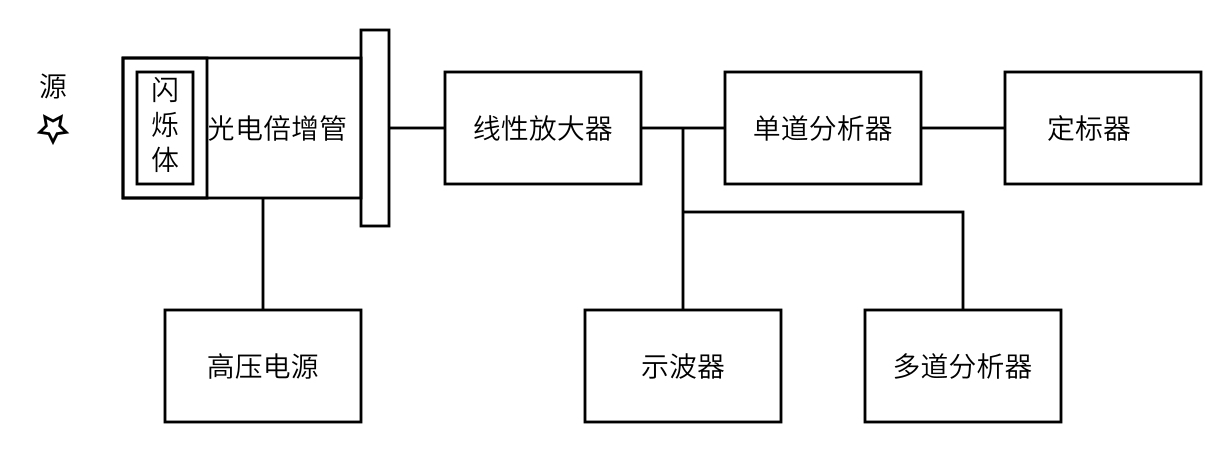
\includegraphics[width=0.45\textwidth]{tu1.png}
\\
\xiaowu\song 图~1\begin{minipage}[t]{75mm} \quad 测量$\gamma$能谱装置仪器示意图。由源,闪烁体探测器以及后续放大分析的电子学器件组成。\\[-1mm]\wuhao
\end{minipage}
\end{center}

本实验中的闪烁体探测器采用的是NaI(Tl)闪烁体,采用$^{137}$Cs作为放射源。放射源产生的$\gamma$射线在闪烁体中发生光电效应和康普顿效应,产生的电子与闪烁体内的物质反应发出光信号,经过光电被增管转化为电信号并有射极跟随器输出。探测器的输出信号则经过线性放大器放大后进入单道或者多道从而对数据进行分析。

实验过程如下
\begin{enumerate}
\item 按照图1连接实验装置,将Cs源放置在托盘上并紧贴闪烁体探测器,将示波器接入电路,调节选择合适的高压(700V左右)以及放大倍数,使得示波器中能够看到经过线性放大器输出的信号。
\item 结合单道调整放大倍数,使得单能峰落在7V附近,并利用单道测量Cs源的能谱。
\item 而后对测量仪器进行标定。首先将放大倍数缩小一倍,测量能量为0.662MeV的全能峰以及0.184MeV的反散射峰对应的阈值电压。然后换上$^{60}$Co源并测量它的两个光电峰对应的阈值电压。用着四个点对探测器进行标定。
\item 使用多道直接测量$^{137}$Cs和$^{60}$Co的混合能谱以及$^{137}$Cs的能谱。
\end{enumerate}


\section{实验结果和讨论}

调整探测器的高压为700V,随后确定放大倍数。利用多道和定标器测量输出电压在6.7V-7.2V附近3s内的计数,细致的调整放大倍数使得峰值出现在7V左右。这时选定的放大倍数为16.4倍。随后在这个条件下测量Cs的全能谱。测量时间为30s每数据点。数据表如下:

\begin{center}
\bgliu
{\bf 表~1\quad
Cs全能谱。 阈值为单道阈值电压值,计数测量时间为30s/数据点,线性放大器放大倍数为16.4}\\[0.5mm]
\renewcommand{\arraystretch}{1.5}
\liuhao\song\rm
\newcolumntype{M}{>{\centering\arraybackslash}m{10mm} >{\centering\arraybackslash}m{7.5mm}
>{\centering\arraybackslash}m{10mm}>{\centering\arraybackslash}m{7.5mm}>{\centering\arraybackslash}m{10mm}>{\centering\arraybackslash}m{7.5mm}}
\begin{tabular}{M}
\specialrule{0.1em}{1pt}{1pt}

阈值/V  &  计数 &  阈值/V  &  计数 &  阈值/V  &  计数 \\
\midrule
8.0   &  150   &  5.5   &  856   &  3.0   &  3986  \\
7.9   &  172   &  5.4   &  1031  &  2.9   &  4039  \\
7.8   &  249   &  5.3   &  1279  &  2.8   &  4190  \\
7.7   &  463   &  5.2   &  1597  &  2.7   &  4175  \\
7.6   &  1052  &  5.1   &  2103  &  2.6   &  4325  \\
7.5   &  2158  &  5.0   &  2780  &  2.5   &  4540  \\
7.4   &  4585  &  4.9   &  3230  &  2.4   &  4727  \\
7.3   &  8068  &  4.8   &  3557  &  2.3   &  4889  \\
7.2   &  12813 &  4.7   &  3811  &  2.2   &  4999  \\
7.1   &  16489 &  4.6   &  3873  &  2.1   &  4945  \\
7.0   &  18521 &  4.5   &  3752  &  2.0   &  4737  \\
6.9   &  18295 &  4.4   &  3705  &  1.9   &  4188  \\
6.8   &  15964 &  4.3   &  3655  &  1.8   &  3978  \\
6.7   &  12116 &  4.2   &  3624  &  1.7   &  3899  \\
6.6   &  8504  &  4.1   &  3751  &  1.6   &  3731  \\
6.5   &  5419  &  4.0   &  3695  &  1.5   &  3847  \\
6.4   &  3780  &  3.9   &  3726  &  1.4   &  3717  \\
6.3   &  2556  &  3.8   &  3617  &  1.3   &  3711  \\
6.2   &  1841  &  3.7   &  3575  &  1.2   &  3719  \\
6.1   &  1466  &  3.6   &  3624  &  1.1   &  3769  \\
6.0   &  1050  &  3.5   &  3779  &  1.0   &  3858  \\
5.9   &  873   &  3.4   &  3770  &  0.9   &  3839  \\
5.8   &  717   &  3.3   &  3693  &  0.8   &  3878  \\
5.7   &  710   &  3.2   &  3724  &  -  &  -  \\
5.6   &  735   &  3.1   &  3786  &  -  &  -  \\
\specialrule{0.1em}{3pt}{2pt}\\[-4mm]
\end{tabular}\\
\renewcommand{\arraystretch}{1.0}
\end{center}

可以看出全能峰和反散射峰分别出现在2.2V和7.0V左右。全能图如下:


\begin{center}
   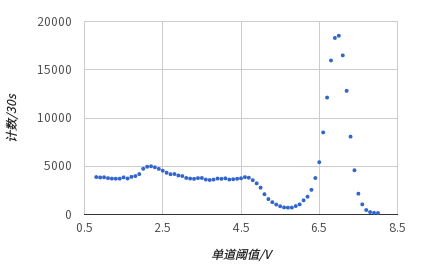
\includegraphics[width=0.4\textwidth]{quanneng.png}
\\
\xiaowu\song 图~2\begin{minipage}[t]{75mm} \quad Cs全能图。可以看出全能峰位于约7V处,反散射峰位于约2.2V处。阈值为单道阈值电压值,计数测量时间为30s/数据点,线性放大器放大倍数为16.4\\[-1mm]\wuhao
\end{minipage}
\end{center}

随后便可以通过Cs源以及Co源对该探测器进行能量刻度了。将放大倍数缩小一倍,这样Co的两个光电峰(1.17MeV, 1.33MeV)才能被单道观察到。此时放大倍数为8.2倍。测量得到的数据如下:

\begin{center}
\bgliu
{\bf 表~2\quad
探测器标定,$^{137}$Cs全能峰位置测量。放大倍数为0.82,测量时间为30s}\\[0.5mm]
\renewcommand{\arraystretch}{1.5}
\liuhao\song\rm
\newcolumntype{M}{>{\centering\arraybackslash}m{10mm} >{\centering\arraybackslash}m{7.5mm}
>{\centering\arraybackslash}m{7.5mm}>{\centering\arraybackslash}m{7.5mm}>{\centering\arraybackslash}m{7.5mm}>{\centering\arraybackslash}m{7.5mm}}
\begin{tabular}{M}
\specialrule{0.1em}{1pt}{1pt}

阈值/V  &  3.3 &  3.4  &  3.5 &  3.6  &  3.7 \\
\midrule
计数   &  12515 &
24294&
31998&
24702&
10475\\
\specialrule{0.1em}{3pt}{2pt}\\[-4mm]
\end{tabular}\\
\renewcommand{\arraystretch}{1.0}
\end{center}


\begin{center}
\bgliu
{\bf 表~3\quad
探测器标定,$^{137}$Cs反散射峰位置测量。放大倍数为0.82,测量时间为30s}\\[0.5mm]
\renewcommand{\arraystretch}{1.5}
\liuhao\song\rm
\newcolumntype{M}{>{\centering\arraybackslash}m{10mm} >{\centering\arraybackslash}m{7.5mm}
>{\centering\arraybackslash}m{7.5mm}>{\centering\arraybackslash}m{7.5mm}>{\centering\arraybackslash}m{7.5mm}>{\centering\arraybackslash}m{7.5mm}}
\begin{tabular}{M}
\specialrule{0.1em}{1pt}{1pt}

阈值/V  &  0.9 &  1.0  &  1.1 &  1.2  &  1.3 \\
\midrule
计数   &  7576 &
8586&
9223&
8610&
8004\\
\specialrule{0.1em}{3pt}{2pt}\\[-4mm]
\end{tabular}\\
\renewcommand{\arraystretch}{1.0}
\end{center}


\begin{center}
\bgliu
{\bf 表~4\quad
探测器标定,$^{60}$Co1.17MeV光电峰位置测量。放大倍数为0.82,测量时间为30s}\\[0.5mm]
\renewcommand{\arraystretch}{1.5}
\liuhao\song\rm
\newcolumntype{M}{>{\centering\arraybackslash}m{10mm} >{\centering\arraybackslash}m{7.5mm}
>{\centering\arraybackslash}m{7.5mm}>{\centering\arraybackslash}m{7.5mm}>{\centering\arraybackslash}m{7.5mm}>{\centering\arraybackslash}m{7.5mm}}
\begin{tabular}{M}
\specialrule{0.1em}{1pt}{1pt}

阈值/V  &  5.7 &  5.8  &  5.9 &  6.0  &  6.1 \\
\midrule
计数   &  1164&
1484&
1798&
1756&
1353\\
\specialrule{0.1em}{3pt}{2pt}\\[-4mm]
\end{tabular}\\
\renewcommand{\arraystretch}{1.0}
\end{center}


\begin{center}
\bgliu
{\bf 表~5\quad
探测器标定,$^{60}$Co1.33MeV光电峰位置测量。放大倍数为0.82,测量时间为30s}\\[0.5mm]
\renewcommand{\arraystretch}{1.5}
\liuhao\song\rm
\newcolumntype{M}{>{\centering\arraybackslash}m{10mm} >{\centering\arraybackslash}m{7.5mm}
>{\centering\arraybackslash}m{7.5mm}>{\centering\arraybackslash}m{7.5mm}>{\centering\arraybackslash}m{7.5mm}>{\centering\arraybackslash}m{7.5mm}}
\begin{tabular}{M}
\specialrule{0.1em}{1pt}{1pt}

阈值/V  &  6.5 &  6.6  &  6.7 &  6.8  &  6.9 \\
\midrule
计数   &  985&
1291&
1306&
1096&gma
654\\
\specialrule{0.1em}{3pt}{2pt}\\[-4mm]
\end{tabular}\\
\renewcommand{\arraystretch}{1.0}
\end{center}

从表格中可以看出,在放大倍数缩小了一倍后,Cs对应电压的计数数目增加了大约0.8倍。这一点很好解释,因为放大倍数缩小一倍,0.1V的道宽对应的能谱宽度是增加了一倍,因而计数增加,峰宽变窄。将四个标定数据集合后再进行拟合就可以得到最终的标定结果。如图3所示,最终的标定结果为
\begin{equation}
   E = 0.206 U - 0.047 
\end{equation}
其中E为能量,单位为MeV,U为阈值电压,单位为V。这个对应着放大倍数为8.2时的标定结果。

\begin{center}
   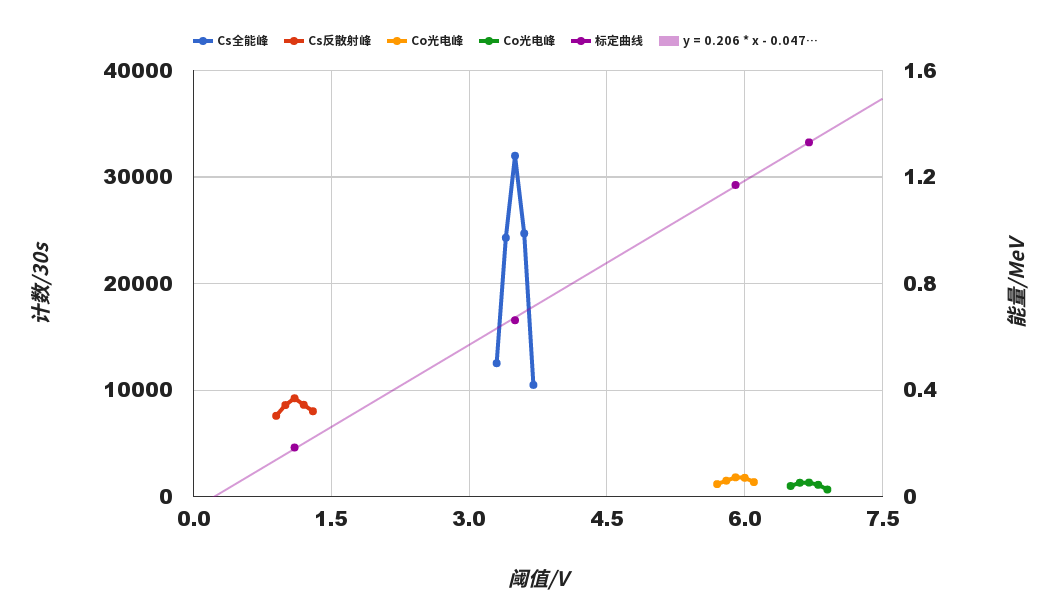
\includegraphics[width=0.48\textwidth]{ALLINONE.png}
\\
\xiaowu\song 图~3\begin{minipage}[t]{75mm} \quad 利用Cs和Co进行能量刻度数据图。计数时间为30s。放大倍数为8.2倍\\[-1mm]\wuhao
\end{minipage}
\end{center}

随后利用多道测量Co和Cs的混合能谱以及Cs的全能谱。因为源的问题,Cs源的强度要远大于Co的强度,因而需要将Cs防止在合适的位置(稍微远离探测器,放置在探测器底部底板上)这样的话混合能谱能够较为清晰的呈现。利用多道获得的能谱如下图4,5,6。

\begin{center}
   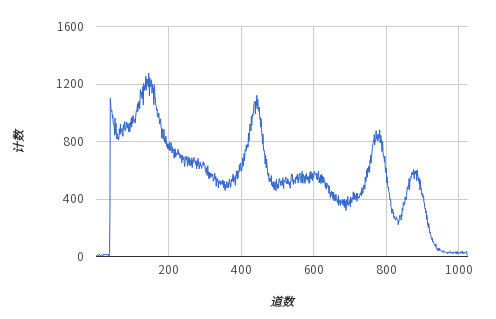
\includegraphics[width=0.48\textwidth]{CSCO.png}
\\
\xiaowu\song 图~4\begin{minipage}[t]{75mm} \quad $^{60}$Co+$^{137}$Cs能谱图。测量时间5min。\\[-1mm]\wuhao
\end{minipage}
\end{center}
\begin{center}
   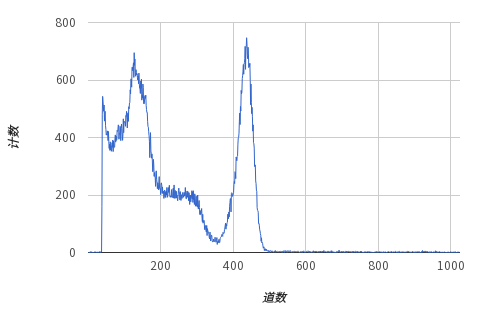
\includegraphics[width=0.48\textwidth]{CS.png}
\\
\xiaowu\song 图~5\begin{minipage}[t]{75mm} \quad $^{137}$Cs能谱图。测量时间5min。\\[-1mm]\wuhao
\end{minipage}
\end{center}
\begin{center}
   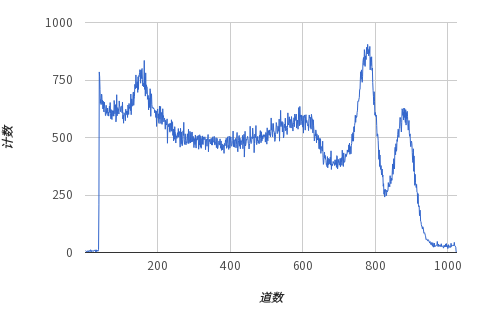
\includegraphics[width=0.48\textwidth]{CO.png}
\\
\xiaowu\song 图~6\begin{minipage}[t]{75mm} \quad $^{60}$Co能谱图。测量时间5min。\\[-1mm]\wuhao
\end{minipage}
\end{center}

对比而言,混合谱就是两个分离谱的叠加,Cs的反散射峰在126道,Co的反散射峰(两个反散射峰比较接近,因分辨率而不能区分)在154道,同时因为两者的反散射峰半宽都很大,探测器分辨率不太好,因而当合并在一起的时候不能区分,在144道形成了一个更大的反散射峰。同样的对比放置在底座上Cs的能谱和放置在托架上的Cs能谱可以发现,反散射峰的强度变强而全能峰的强度便弱。这个也是很好解释的,因为放射源离探测器远了,所以全能峰计数肯定会降低。同时反散射峰有一部分是来自于底座金属的散射,因为源离底座更近了,所以反散射加强,从而反散射峰的计数增多。

\section{总结和结论}
本次实验中,通过NaI闪烁体谱仪测量了$^{137}$Cs的能谱,得到的能谱图如图一所示。并利用Cs和Co对该探测器进行了标定,标定结果为$  E = 0.206 U - 0.047 $(MeV)。最后利用多道研究了$^{137}$Cs以及$^{60}$Co的能谱,能谱图如图四,五,六所示。
\section{致谢}
感谢楼建玲老师的细致地讲解以及为实验做出的准备。
\section{参考文献}

\noindent
[1] Peking Unviersity, Fudan University \ Nuclear Experment
\ Nuclear Publishing House, 1989: 87-95. (in Chinese)

\noindent
 (北京大学,复旦大学.\ 原子核实验\ 原子能出版社,\ 1989: 87-95.)

\noindent
[2] 讲义
\end{multicols}

\newpage


\section*{附录:思考题}
1、能量刻度是将探测器输出的电压值和实际粒子能量关联起来的途径,没有能量刻度测量值不能代表粒子的能量。本实验中使用了Cs和Co的已知能量的4个峰进行刻度。当放射源不够多时,可以利用放射源能谱中一些固有的峰位进行刻度,比如利用反散射峰等。

2、将经放大器输出的信号接入示波器既可以看到脉冲波形图。谱仪能量分辨率好的话示波器上看到的全能峰应该明亮锐利。如果不是特别的锐利表明分辨率不是太好。

3、测量时间根据信号多少来选取,对于一个强的源产生粒子多信号多就可以时间选短一些。主要考虑的因素是减弱因统计而带来的误差。为了精确测量能量分辨率则应选取单能性较好的源,并且排除其他的噪声污染(附近不要放其他源),以及在时间选择上应该保证测量时间足够长到Cs的全能峰是一个较好高斯峰,道宽则应该选择精细到能够清晰的观察到全能峰的形状。

4、应该使得全能峰落在单道的范围内,即能够利用单道完全的观测到全能峰。道宽选择应该在保证统计误差影响不大的情况下尽量减少。阈值改变量则应等于道宽。

5、反散射峰是$\gamma$光子与电子发生康普顿散射后被完全反向弹回,被弹回的光子进入闪烁体后形成的信号。减小反散射峰则应避免在源周围放置自由电子较多的材料,比如说使用塑料作为源的支架材料。

\clearpage
%\end{CJK*}
\end{document}

